\documentclass[12pt]{report}
\usepackage[utf8]{inputenc}
\usepackage[russian]{babel}
%\usepackage[14pt]{extsizes}
\usepackage{listings}

\usepackage{graphicx}
\graphicspath{{src/}}
\DeclareGraphicsExtensions{.pdf,.png,.jpg}

\usepackage{amsmath,amsfonts,amssymb,amsthm} 

% Для листинга кода:
\lstset{ %
language=c++,                 % выбор языка для подсветки (здесь это С++)
basicstyle=\small\sffamily, % размер и начертание шрифта для подсветки кода
numbers=left,               % где поставить нумерацию строк (слева\справа)
numberstyle=\tiny,           % размер шрифта для номеров строк
stepnumber=1,                   % размер шага между двумя номерами строк
numbersep=5pt,                % как далеко отстоят номера строк от подсвечиваемого кода
showspaces=false,            % показывать или нет пробелы специальными отступами
showstringspaces=false,      % показывать или нет пробелы в строках
showtabs=false,             % показывать или нет табуляцию в строках
frame=single,              % рисовать рамку вокруг кода
tabsize=2,                 % размер табуляции по умолчанию равен 2 пробелам
captionpos=t,              % позиция заголовка вверху [t] или внизу [b] 
breaklines=true,           % автоматически переносить строки (да\нет)
breakatwhitespace=false, % переносить строки только если есть пробел
escapeinside={\#*}{*)}   % если нужно добавить комментарии в коде
}

% Для измененных титулов глав:
\usepackage{titlesec, blindtext, color} % подключаем нужные пакеты
\definecolor{gray75}{gray}{0.75} % определяем цвет
\newcommand{\hsp}{\hspace{20pt}} % длина линии в 20pt
% titleformat определяет стиль
\titleformat{\chapter}[hang]{\Huge\bfseries}{\thechapter\hsp\textcolor{gray75}{|}\hsp}{0pt}{\Huge\bfseries}


% plot
\usepackage{pgfplots}
\usepackage{filecontents}
\usetikzlibrary{datavisualization}
\usetikzlibrary{datavisualization.formats.functions}


\begin{document}
\begin{titlepage}
	\centering
	{\scshape\LARGE МГТУ им. Баумана \par}
	\vspace{3cm}
	{\scshape\Large Лабораторная работа №2\par}
	\vspace{0.5cm}	
	{\scshape\Large По курсу: "Анализ алгоритмов"\par}
	\vspace{1.5cm}
	{\huge\bfseries Алгоритмы умножения матриц\par}
	\vspace{2cm}
	\Large Работу выполнил: Чернов Даниил, ИУ7-56Б\par
	\vspace{0.5cm}
	\LargeПреподаватели:  Волкова Л.Л., Строганов Ю.В.\par

	\vfill
	\large \textit {Москва, 2019} \par
\end{titlepage}

\tableofcontents

\newpage
\chapter*{Введение}
\addcontentsline{toc}{chapter}{Введение}
Цель работы: изучение алгоритмов умножения матриц. В данной лабораторной работе рассматривается стандартный алгоритм умножения матриц, алгоритм Винограда и модифицированный алгоритм Винограда.  Также требуется изучить рассчет сложности алгоритмов, получить навыки в улучшении алгоритмов.


В ходе лабораторной работы предстоит решить следующие задачи:
\begin{itemize}
	\item изучить алгоритмы умножения матриц: стандартный и алгоритм Винограда; 
	\item оптимизировать алгоритм Винограда; 
	\item дать теоретическую оценку базового алгоритма умножения матриц, алгоритма Винограда и улучшенного алгоритма Винограда;
	\item реализовать три алгоритма умножения матриц на одном из языков программирования;  
	\item сравнить алгоритмы умножения матриц.
\end{itemize}



\chapter{Аналитическая часть}
Матрицей A размера $[m*n]$ называется прямоугольная таблица
чисел, функций или алгебраических выражений, содержащая m строк и n столбцов. Числа m и n определяют размер матрицы.\cite{Beloysov} Если число столбцов в первой матрице совпадает с числом строк во второй, то эти две матрицы можно перемножить. У произведения будет столько же строк, сколько в первой матрице, и столько же столбцов, сколько во второй.
	    
Пусть даны две прямоугольные матрицы А и В размеров $[m * n]$ и $[n * k]$ соответственно.  
В результате произведение матриц A и B получим матрицу C размера $[m *  k]$.

$C_{i,j} = \sum\limits_{r=1}^n A_{i,r}\cdot B_{r,j}$ называется произведением матриц A и B \cite{Beloysov}.


\section{Алгоритм Винограда}
Подход Алгоритма Винограда является иллюстрацией общей методологии, начатой в 1979-х годах на основе
билинейных и трилинейных форм, благодаря которым большинство усовершенствований для умножения матриц были получены \cite{Gall2012}.

Рассмотрим два вектора $V = (v1, v2, v3, v4)$ и $W = (w1, w2, w3, w4)$.  

 Их скалярное произведение равно (\ref{formula}) 

\begin{equation} \label{formula}
V \cdot W=v_1 \cdot w_1 + v_2 \cdot w_2 + v_3 \cdot w_3 + v_4 \cdot w_4
\end{equation}

Равенство (\ref{formula}) можно переписать в виде (\ref{formula2}) 
\begin{equation} \label{formula2}
V \cdot W=(v_1 + w_2) \cdot (v_2 + w_1) + (v_3 + w_4) \cdot (v_4 + w_3) - v_1 \cdot v_2 - v_3 \cdot v_4 - w_1 \cdot w_2 - w_3 \cdot w_4
\end{equation}

Выражение в правой части последнего равенства допускает предварительную обработку: его части можно вычислить заранее и запомнить для каждой строки первой матрицы и для каждого столбца второй. 
Это означает, что над предварительно обработанными элементами нам придется выполнять лишь первые два умножения и последующие пять сложений, а также дополнительно два сложения. 

В алгоритме Винограда, результатом умножение матриц A размером $[m * n]$ и B размером $[n * k]$ получим матрицу C размера $[m *  k]$ которая вычисляется по следующим формулам:

Вычисление строковых множителей (\ref{rowFactors})
\begin{equation} \label{rowFactors}
Rows_{i} = \sum\limits_{j = 1}^{n/2} A_{i, 2j} \cdot A_{i, 2j+1}
\end{equation}

Вычисление множителей стобцов (\ref{columnFactors})
\begin{equation} \label{columnFactors}
Cols_{i} = \sum\limits_{j = 1}^{n/2} B_{2j, i} \cdot B_{2j+1, i}
\end{equation}

Вычисление результирующей матрицы С (\ref{result})
\begin{equation} \label{result}
C_{i,j} = -Rows_{i} -  Cols_{j} + \sum\limits_{k = 1}^{n/2} (A_{i, 2k+1} + B_{2k, j}) \cdot (A_{i, 2k} + B_{2k+1,j})
\end{equation}

Следует отметить, что в худшем случае (при условии того что кол-во столбцев в матрице А либо кол-во строк в матрице В - нечётное) к результирующей формуле (\ref{result}) применяется следующее выражение (\ref{resultBad})

\begin{equation} \label{resultBad}
C_{i,j} += A_{i, n} \cdot B_{n, j}
\end{equation}


\section{Вывод}
Были рассмотрены алгоритмы классического умножения матриц и алгоритм Винограда, основное отличие которых — наличие предварительной обработки, а также количество операций умножения.



\chapter{Конструкторская часть}
\textbf{Требования к вводу:}
На вход подаются две матрицы
\newline
\textbf{Требования к программе:}
\begin{itemize}
\item корректное умножение двух матриц;
\item при матрицах неправилыных размеров программа не должна аварийно завершаться.
\end{itemize}

\section{Схемы алгоритмов}
В данной части будут рассмотрены схемы алгоритмов.

\begin{figure}[!htbp]
\centering
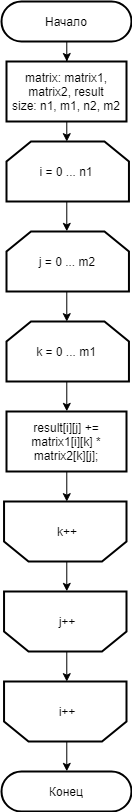
\includegraphics[scale=0.7]{SchemeStand}
\caption{Схема классического алгоритма умножения матриц}
\label{fig:mpr}
\end{figure}

\begin{figure}[!htbp]
\centering
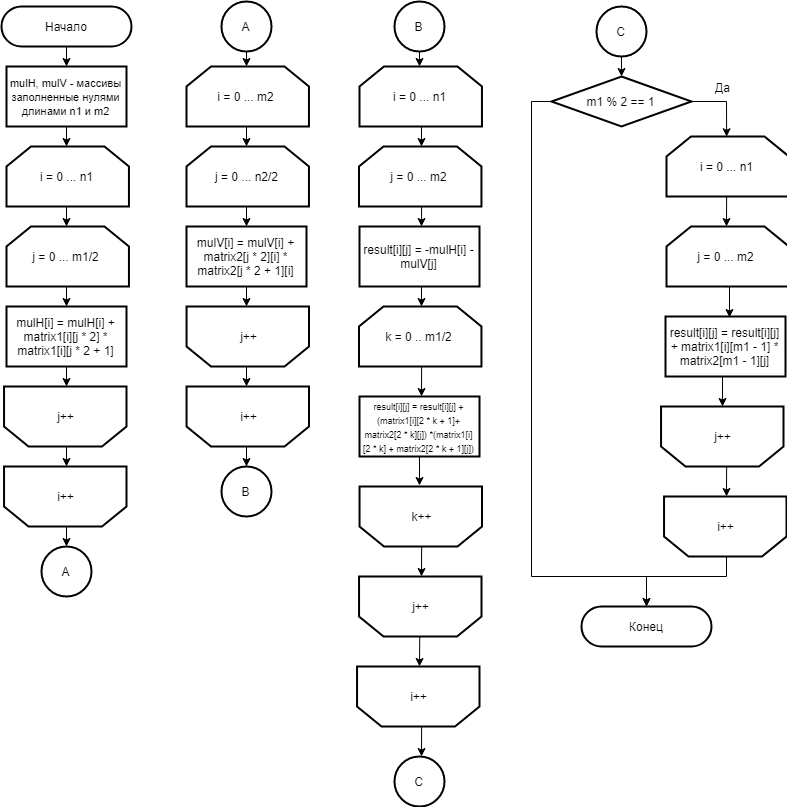
\includegraphics[scale=0.6]{SchemeVin}
\caption{Схема алгоритма Винограда}
\label{fig:mpr}
\end{figure}


\begin{figure}[!htbp]
\centering
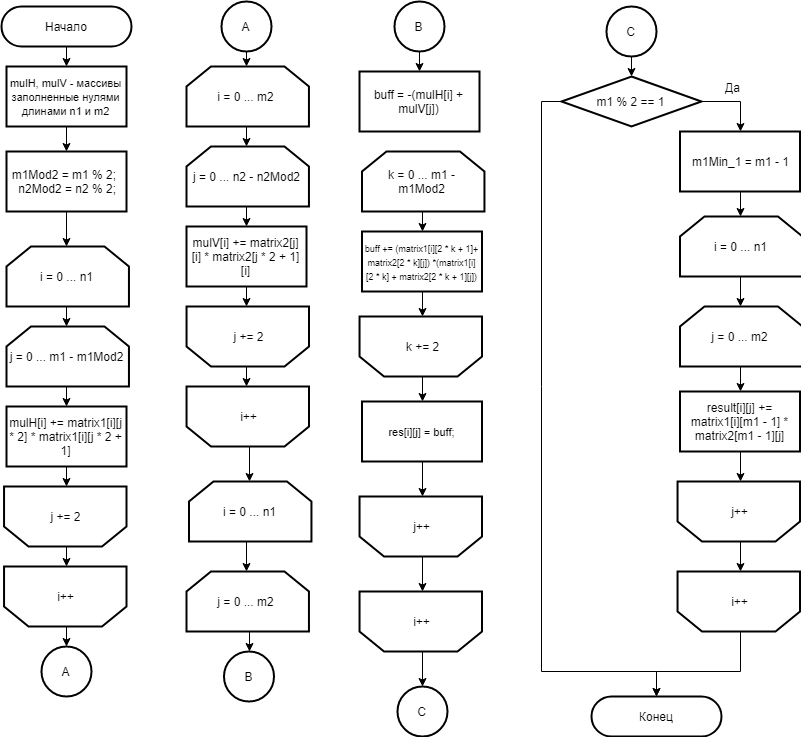
\includegraphics[scale=0.6]{SchemeVinOpt}
\caption{Схема оптимизированного алгоритма Винограда}
\label{fig:mpr}
\end{figure}

\newpage
\section{Трудоемкость алгоритмов}
Введем модель трудоемкости для оценки алгоритмов: 
\begin{itemize}
	\item базовые операции стоимостью 1 — +, -, *, /, =, ==, <=, >=, !=, +=, [], получение полей класса
	\item оценка трудоемкости цикла: Fц = init +  N*(a + Fтела + post) + a, где a - условие цикла, init - предусловие цикла, post - постусловие цикла
	\item стоимость условного перехода применим за 0, стоимость вычисления условия остаётся
\end{itemize}

Оценим трудоемкость алгоритмов по коду программы.

\subsection{Трудоемкость первичной проверки}
Рассмотрим трудоемкость первичной проверки на возможность умножения матриц.

\begin{center}
Табл. 2.1 Построчная оценка веса
	\begin{tabular}{|l c|} 
 	\hline
	Код & Вес \\ [0.5ex] 
 	\hline\hline
 	int firstRowCount = firstMatrix.length; & 2\\
 	\hline
	int secondRowCount = secondMatrix.length; & 2\\
	\hline
	if (firstRowCount == 0 || secondRowCount == 0) return null; & 3\\
	\hline
	int firstColumnCount = firstMatrix[0].length; & 3\\
	\hline
	int secondColumnCount = secondMatrix[0].length; & 3\\
	\hline
	if (firstColumnCount == 0 || secondColumnCount == 0) return null; & 1\\
	\hline\hline
	Итого & 14\\
	\hline
	\end{tabular}
\end{center}

\subsection{Классический алгоритм}
Рассмотрим трудоемкость классического алгоритма:  

Инициализация матрицы результата: $1 + 1 + n_1(1 + 2 + 1) + 1 = 4n_1 + 3$

Подсчет:\\
$1 + n_1(1 + (1 + m_2(1 + (1 + m_1(1 + (8) + 1) + 1) + 1) + 1) + 1) + 1 = 
n_1(m_2(10m_1 + 4) + 4) + 4) + 2 = 10n_1m_2m_1+ 4n_1m_2 + 4n_1 +2
$

\subsection{Алгоритм Винограда}
Аналогично рассмотрим трудоемкость алгоритма Винограда.  \\

Первый цикл: $\frac{15}{2}n_1m_1 + 5n_1 + 2$ 

Второй цикл: $\frac{15}{2}m_2n_2+ 5m_2 + 2$

Третий цикл: $13n_1m_2m_1 + 12n_1m_2 + 4n_1 + 2$

Условный переход: $\begin{bmatrix}
             2    &&, \text{невыполнение условия}\\
             15n_1m_2 + 4n_1 + 2 &&, \text{выполнение условия}\\
           \end{bmatrix} $ \\

Итого: $  13n_1m_2m_1 + \frac{15}{2}n_1m_1 +\frac{15}{2}m_2n_2 + 12n_1m_2 + 5n_1 + 5m_2 + 4n_1 + 6 + \\
       \begin{bmatrix}
             2    &&, \text{невыполнение условия}\\
             15n_1m_2 + 4n_1 + 2 &&, \text{выполнение условия}\\
           \end{bmatrix} $ \\

\subsection{Оптимизированный алгоритм Винограда}

Аналогично Рассмотрим трудоемкость оптимизированого алгоритма Винограда:\\

Первый цикл: $\frac{11}{2}n_1m_1 + 4n_1 + 2$ 

Второй цикл: $\frac{11}{2}m_2n_2+ 4m_2 + 2$

Третий цикл: $\frac{17}{2}n_1m_2m_1 + 9n_1m_2 + 4n_1 + 2$

Условный переход: $\begin{bmatrix}
             1    &&, \text{невыполнение условия}\\
             10n_1m_2 + 4n_1 + 2 &&, \text{выполнение условия}\\
           \end{bmatrix} $ \\

Итого: $\frac{17}{2}n_1m_2m_1 + \frac{11}{2}n_1m_1 + \frac{11}{2}m_2n_2 + 9n_1m_2 + 8n_1 + 4m_2 + 6 + \\
       \begin{bmatrix}
             1    &&, \text{невыполнение условия}\\
             10n_1m_2 + 4n_1 + 2 &&, \text{выполнение условия}\\
           \end{bmatrix} $ \\

\section{Вывод}
В данном разделе были рассмотрены схемы алгоритмов умножения матриц, введена модель оценки трудоемкости алгоритма, были расчитаны трудоемкости алгоритмов в соответсвии с этой моделью.



\chapter{Технологическая часть}
\section{Выбор ЯП}
В качестве языка программирования был выбран Java \cite{Microsoft}, а средой разработки Intellij IDEA. 
Время работы алгоритмов было замерено с помощью класса System.Time.


\section{Сведения о модулях программы}
Программа состоит из:
\begin{itemize}
	\item Main.java - главный файл программы, в котором располагается точка входа в программу и функция замера времени.
	\item MatrixMultiplication.java - класс, реализующий стандартный алгоритм умножения матриц.
	\item WinogradMultiplication.java - класс, реализующий алгоритм умножения матриц по Винограду.
	\item WinogradOpimizedMultiplication.java - класс, реализующий улачшенный алгоритм Винограда для умножения матриц.
	\item RandomMatrix.java - класс, реализующий генерацию случайных матрицы заданного размера.
	\item TestCases.java - класс, реализовующий юнит-тестирование.
\end{itemize}


\section{Листинг кода алгоритмов}
В листингах 3.1 - 3.3 будет рассмотрена реализация описанных алгоритмов.

\begin{lstlisting}[label=CodeStand,caption= Стандартный алгоритм умножения матриц]
public class MatrixMultiplication {
    static public int[][] Multiply(@NotNull int[][] matrixA, @NotNull int[][] matrixB) {
        if (matrixA.length == 0 || matrixB.length == 0)
            return null;
        if (matrixA[0].length != matrixB.length)
            return null;

        int[][] matrixResult = new int[matrixA.length][matrixB[0].length];

        for (int i = 0; i < matrixA.length; i++)
            for (int j = 0; j < matrixB[0].length; j++)
                for (int k = 0; k < matrixB.length; k++)
                    matrixResult[i][j] = matrixResult[i][j] + matrixA[i][k] * matrixB[k][j];
        return matrixResult;
    }
}
\end{lstlisting}


\begin{lstlisting}[label=some-code,caption=Алгоритм Винограда]
public class WinogradMultiplication extends MatrixMultiplication {
    static public int[][] Multiply(@NotNull int[][] matrixA, @NotNull int[][] matrixB) {
        if (matrixA.length == 0 || matrixB.length == 0)
            return null;
        if (matrixA[0].length != matrixB.length)
            return null;

        int[][] matrixResult = new int[matrixA.length][matrixB[0].length];
        int firstRowCount = matrixA.length;
        int firstColumnCount = matrixA[0].length;
        int secondRowCount = matrixB.length;
        int secondColumnCount = matrixB[0].length;
        int[] rowFactor = new int[firstRowCount];
        int[] columnFactor = new int[secondColumnCount];

        for(int i = 0; i < firstRowCount; i++)
            for (int j = 0; j < firstColumnCount / 2; j++)
                rowFactor[i] += matrixA[i][2 * j] * matrixA[i][2 * j + 1];

        for(int i = 0; i < secondColumnCount; i++)
            for (int j = 0; j < secondRowCount / 2; j++)
                columnFactor[i] += matrixB[2 * j][i] * matrixB[2 * j + 1][i];

        for(int i = 0; i < firstRowCount; i++)
            for(int j = 0; j < secondColumnCount; j++) {
                matrixResult[i][j] = -rowFactor[i] - columnFactor[j];
                for(int k = 0; k < firstColumnCount / 2; k++)
                    matrixResult[i][j] += + (matrixA[i][2 * k + 1] + matrixB[2 * k][j]) *
                            (matrixA[i][2 * k] + matrixB[2 * k + 1][j]);
            }

        if (firstColumnCount % 2 == 1)
            for (int i = 0; i < firstRowCount; i++)
                for (int j = 0; j < secondColumnCount; j++)
                    matrixResult[i][j] += matrixA[i][firstColumnCount - 1] * matrixB[firstColumnCount - 1][j];

        return matrixResult;
    }
}
\end{lstlisting}


\begin{lstlisting}[label=some-code,caption=Оптимизированный алгоритм Винограда]
public class WinogradOptimizedMultiplication extends WinogradMultiplication {
    static public int[][] Multiply(@NotNull int[][] matrixA, @NotNull int[][] matrixB) {
        if (matrixA.length == 0 || matrixB.length == 0)
            return null;
        if (matrixA[0].length != matrixB.length)
            return null;

        int[][] matrixResult = new int[matrixA.length][matrixB[0].length];
        int firstRowCount = matrixA.length;
        int secondRowCount = matrixB.length;
        int firstColumnCount = matrixA[0].length;
        int secondColumnCount = matrixB[0].length;
        int[] rowFactors = new int[firstRowCount];
        int[] columnFactors = new int[secondColumnCount];
        int fColumnMod2 = firstColumnCount % 2;
        int sRowMod2 = secondRowCount % 2;

        for (int i = 0; i < firstRowCount; i++)
            for (int j = 0; j < (firstColumnCount - fColumnMod2); j += 2)
                rowFactors[i] += matrixA[i][j] * matrixA[i][j + 1];

        for (int i = 0; i < secondColumnCount; i++)
            for (int j = 0; j < (secondRowCount - sRowMod2); j += 2)
                columnFactors[i] += matrixB[j][i] * matrixB[j + 1][i];

        for (int i = 0; i < firstRowCount; i++)
            for (int j = 0; j < secondColumnCount; j++) {
                int buff = -(rowFactors[i] + columnFactors[j]);
                for (int k = 0; k < (firstColumnCount - fColumnMod2); k += 2)
                    buff += (matrixA[i][k + 1] + matrixB[k][j]) * (matrixA[i][k] + matrixB[k + 1][j]);
                matrixResult[i][j] = buff;
            }

        if (fColumnMod2 == 1)
            for (int i = 0; i < firstRowCount; i++)
                for (int j = 0; j < secondColumnCount; j++)
                    matrixResult[i][j] += matrixA[i][firstColumnCount - 1] * matrixB[firstColumnCount - 1][j];

        return matrixResult;
    }
}

\end{lstlisting}

\subsection{Оптимизация алгоритма Винограда}
В рамках данной лабораторной работы было предложено 3 оптимизации:
\begin{enumerate}
	\item Избавление от деления в условии цикла;
	\item Замена $rowFactors[i] += …$ на $rowFactors[i] += …$ (аналогично для $columnFactors[i]$);
	
\newpage
\begin{lstlisting}[label=some-code,caption=Оптимизации алгоритма Винограда №1 и №2]
	    int fColumnMod2 = firstColumnCount \% 2;
        int sRowMod2 = secondRowCount \% 2;

        for (int i = 0; i < firstRowCount; i++) {
            for (int j = 0; j < (firstColumnCount - fColumnMod2); j += 2) {
                rowFactors[i] += firstMatrix[i][j] * firstMatrix[i][j + 1];
            }
        }

        for (int i = 0; i < secondColumnCount; i++) {
            for (int j = 0; j < (secondRowCount - sRowMod2); j += 2) {
                columnFactors[i] += secondMatrix[j][i] * secondMatrix[j + 1][i];
            }
        }
\end{lstlisting}

\item Накопление результата в буфер, чтобы не обращаться каждый раз к одной и той же ячейке памяти. Сброс буфера в ячейку матрицы после цикла.
\begin{lstlisting}[label=some-code,caption=Оптимизации алгоритма Винограда №3]
    for (int i = 0; i < firstRowCount; i++) {
            for (int j = 0; j < secondColumnCount; j++) {
                int buff = -(rowFactors[i] + columnFactors[j]);
                for (int k = 0; k < (firstColumnCount - fColumnMod2); k += 2) {
                    buff += (firstMatrix[i][k + 1] + secondMatrix[k][j]) * (firstMatrix[i][k] + secondMatrix[k + 1][j]);
                }
                result[i][j] = buff;
            }
        }
\end{lstlisting}
\end{enumerate}

\section{Тестирование программы}

Было произведено тестирование реализованных алгоритмов с помощью библиотеки JUnit.

Всего было реализованно 7 тестовых случаев:
\begin{itemize}
	\item Некорректный размер матриц. Алгоритм должен возвращать Null
	\item Размер матриц равен 0
	\item Размер матриц равен 1
	\item Сравнение работы стандартной реализации с Виноградом на случайных значениях
	\subitem Четный размер
	\subitem Нечетный размер
	\item Сравнение работы стандартной реализации с оптимизированным Виноградом на случайных значениях
	\subitem Четный размер
	\subitem Нечетный размер
\end{itemize}

На \ref{fig:test} будут предоставлены результаты тестирования программы. Откуда видно, что тестирование пройдено, алгоритмы реализованы правильно.
\begin{figure}[!htbp]
\centering
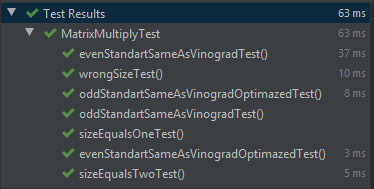
\includegraphics[scale=1.2]{TestsPassed}
\caption{Результаты работы тестов}
\label{fig:test}
\end{figure} 

\newpage
\section{Вывод}
В данном разделе была рассмотрена реализация и тестирование ПО, а так же листинги кода программы.


\chapter{Исследовательская часть}

\section{Сравнительный анализ на основе замеров времени работы алгоритмов}

Был проведен замер времени работы каждого из алгоритмов.

Первый эксперимент производится для лучшего случая на квадратных матрицах размером от 100 x 100 до 1000 x 1000 c шагом 100. 
Сравним результаты для разных алгоритмов:

\begin{tikzpicture}
\begin{axis}[
    	axis lines = left,
    	xlabel = {Размер матрицы},
    	ylabel = {Время (мс)},
	legend pos=north west,
	ymajorgrids=true
]
\addplot[color=red, mark=square] table[x index=0, y index= 1] {src/Stand0.txt}; 
\addplot[color=green, mark=square] table[x index=0, y index= 1] {src/Vin0.txt}; 
\addplot[color=blue, mark=square] table[x index=0, y index= 1] {src/VinOpt0.txt}; 

\addlegendentry{Стандартный}
\addlegendentry{Алг. Винограда}
\addlegendentry{Оптимизированный алг.}

\end{axis}
\end{tikzpicture}
\begin{center}
Pис. 4.1: Сравнение времени работы алгоритмов при четном размере матрицы
\end{center}

\newpage
Второй эксперимент производится для худшего случая, когда поданы квадратные матрицы с нечетными размерами от 101 x 101 до 1001 x 1001 c шагом 100. 
Сравним результаты для разных алгоритмов:

\begin{tikzpicture}
\begin{axis}[
    	axis lines = left,
    	xlabel = {Размер матрицы},
    	ylabel = {Время (мс)},
	legend pos=north west,
	ymajorgrids=true
]
\addplot[color=red, mark=square] table[x index=0, y index= 1] {src/Stand1.txt}; 
\addplot[color=green, mark=square] table[x index=0, y index= 1] {src/Vin1.txt}; 
\addplot[color=blue, mark=square] table[x index=0, y index= 1] {src/VinOpt1.txt}; 

\addlegendentry{Стандартный}
\addlegendentry{Алг. Винограда}
\addlegendentry{Оптимизированный алг.}

\end{axis}
\end{tikzpicture}
\begin{center}
Pис. 4.2: Сравнение времени работы алгоритмов при нечетном размере матрицы
\end{center}


\section{Вывод}
По результатам тестирования все рассматриваемые алгоритмы реализованы правильно. Самым медленным алгоритмом оказался алгоритм классического умножения матриц, а самым быстрым — оптимизированный алгоритм Винограда.

\chapter*{Заключение}
\addcontentsline{toc}{chapter}{Заключение}
В ходе лабораторной работы я изучил алгоритмы умножения матриц: стандартный и Винограда, оптимизировал алгоритм Винограда, дал теоретическую оценку алгоритмов стандартного умножения матриц, Винограда и улучшенного Винограда, реализовал три алгоритма умножения матриц на языке программирования Java и сравнил эти алгоритмы.

\addcontentsline{toc}{chapter}{Список литературы}
 \begin{thebibliography}{3}
\bibitem{Beloysov}
И. В. Белоусов(2006), Матрицы и определители, учебное пособие по линейной алгебре, с. 1 - 16
\bibitem{Gall2012}
Le Gall, F. (2012), "Faster algorithms for rectangular matrix multiplication", Proceedings of the 53rd Annual IEEE Symposium on Foundations of Computer Science (FOCS 2012), pp. 514–523
%https://arxiv.org/pdf/1204.1111.pdf
\bibitem{Oracle Documentation}
Документация по языку Java[Электронный ресурс], - режим доступа: https://docs.oracle.com/en/java/javase/13/
\end{thebibliography}

\end{document}